\chapter{Środowisko symulacyjne}
\label{sec:model}
W tym rozdziale opisane są stworzone składniki systemu, czyli modele dynamiczne i kinematyczne, modele czujników, oraz pakiety wspomagające testowanie.

Aby uruchomić symulację, nie wystarczy uruchomienie symulatora z modelami, należy zadbać także o odpowiednie przekazywanie informacji do i z symulowanych obiektów.
Wskazane jest przetestować modele, czy zachowują się poprawnie w prostych scenariuszach testowych, tak samo, jak testować się będzie program sterujący na modelu.
Do tego potrzebne są programy wspomagające, które łączy się w różne konfiguracje, w zależności od scenariusza testowego.
Ze względu na niezależność pakietów od siebie, można ich także użyć przy komunikacji z rzeczywistym robotem.

Środowisko symulacyjne składa się z kilku odrębnych pakietów, które komunikują się ze sobą poprzez specjalne interfejsy, wykorzystujące kolejki wiadomości.
Taka implementacja komunikacji pozwala zmieniać i reimplementować poszczególne elementy, używać różnych języków programowania, oraz
zachowywać jednolitą komunikację między składnikami i nie tracąc na kompatybilności między pakietami.
Możliwe jest także przesyłanie wiadomości przez sieć, co pozwala na rozproszenie systemu.

Niektóre typy wiadomości posiadają wbudowany nagłówek, inne istnieją w dwóch wersjach, z nagłówkiem i bez. 
Dopisek \texttt{Stamped} określa istnienie tej dodatkowej informacji.
Nagłówek ma trzy pola:
\begin{itemize}
	\item Numer sekwencyjny, zwiększany przez program wysyłający po każdej wysłanej wiadomości.
	\item Czas nadania wiadomości, z dokładnością do nanosekund.
	\item Identyfikator macierzy przekształcenia jednorodnego, według której podano dane, ta funkcjonalność została opisana dokładniej w sekcji \ref{sec:frames}.
\end{itemize}

\begin{table}
	\centering
	\begin{tabular}{l r}
		Typ & Opis \\
		\hline
		\texttt{omnivelma\_msgs/Encoders} & Prędkości i pozycje kół z enkodera. \\
		\texttt{omnivelma\_msgs/Vels} & Prędkości kół. \\
		\texttt{omnivelma\_msgs/SetFriction} & Nadanie tarcia elementowi modelu. \\
		\texttt{omnivelma\_msgs/SetInertia} & Nadanie mas i momentu bezwładności obiektowi. \\
		\texttt{geometry\_msgs/Pose} & Pozycja obiektu w przestrzeni kartezjańskiej. \\
		\texttt{geometry\_msgs/Twist} & Prędkość względna obiektu. \\
		\texttt{sensor\_msgs/LaserScan} & Jedno skanowanie skanera laserowego. \\
		\texttt{omnivelma\_msgs/Relative} & Odległość i kąt pomiędzy obiektami. \\
		\texttt{nav\_msgs/Odometry} & Pozycja obiektu z macierzą kowariancji. \\
		\texttt{sensor\_msgs/Imu} & Dane generowane przez jednostkę inercyjną. \\
	\end{tabular}
	\caption{Typy wiadomości przekazywanych pomiędzy pakietami.}
	\label{tab:messages}
\end{table}

Pakiety można podzielić na trzy typy:
\begin{itemize}
	\item Generujące dane.
	\item Przekazujące i modyfikujące dane.
	\item Zbierające dane.
\end{itemize}
Poniżej, każdy pakiet opisany jest bardziej szczegółowo, wraz z jego interfejsem.

W trakcie testowania symulatora, podłączenie pakietów będzie wyglądać następująco:
\begin{figure}[H]
	\centering
	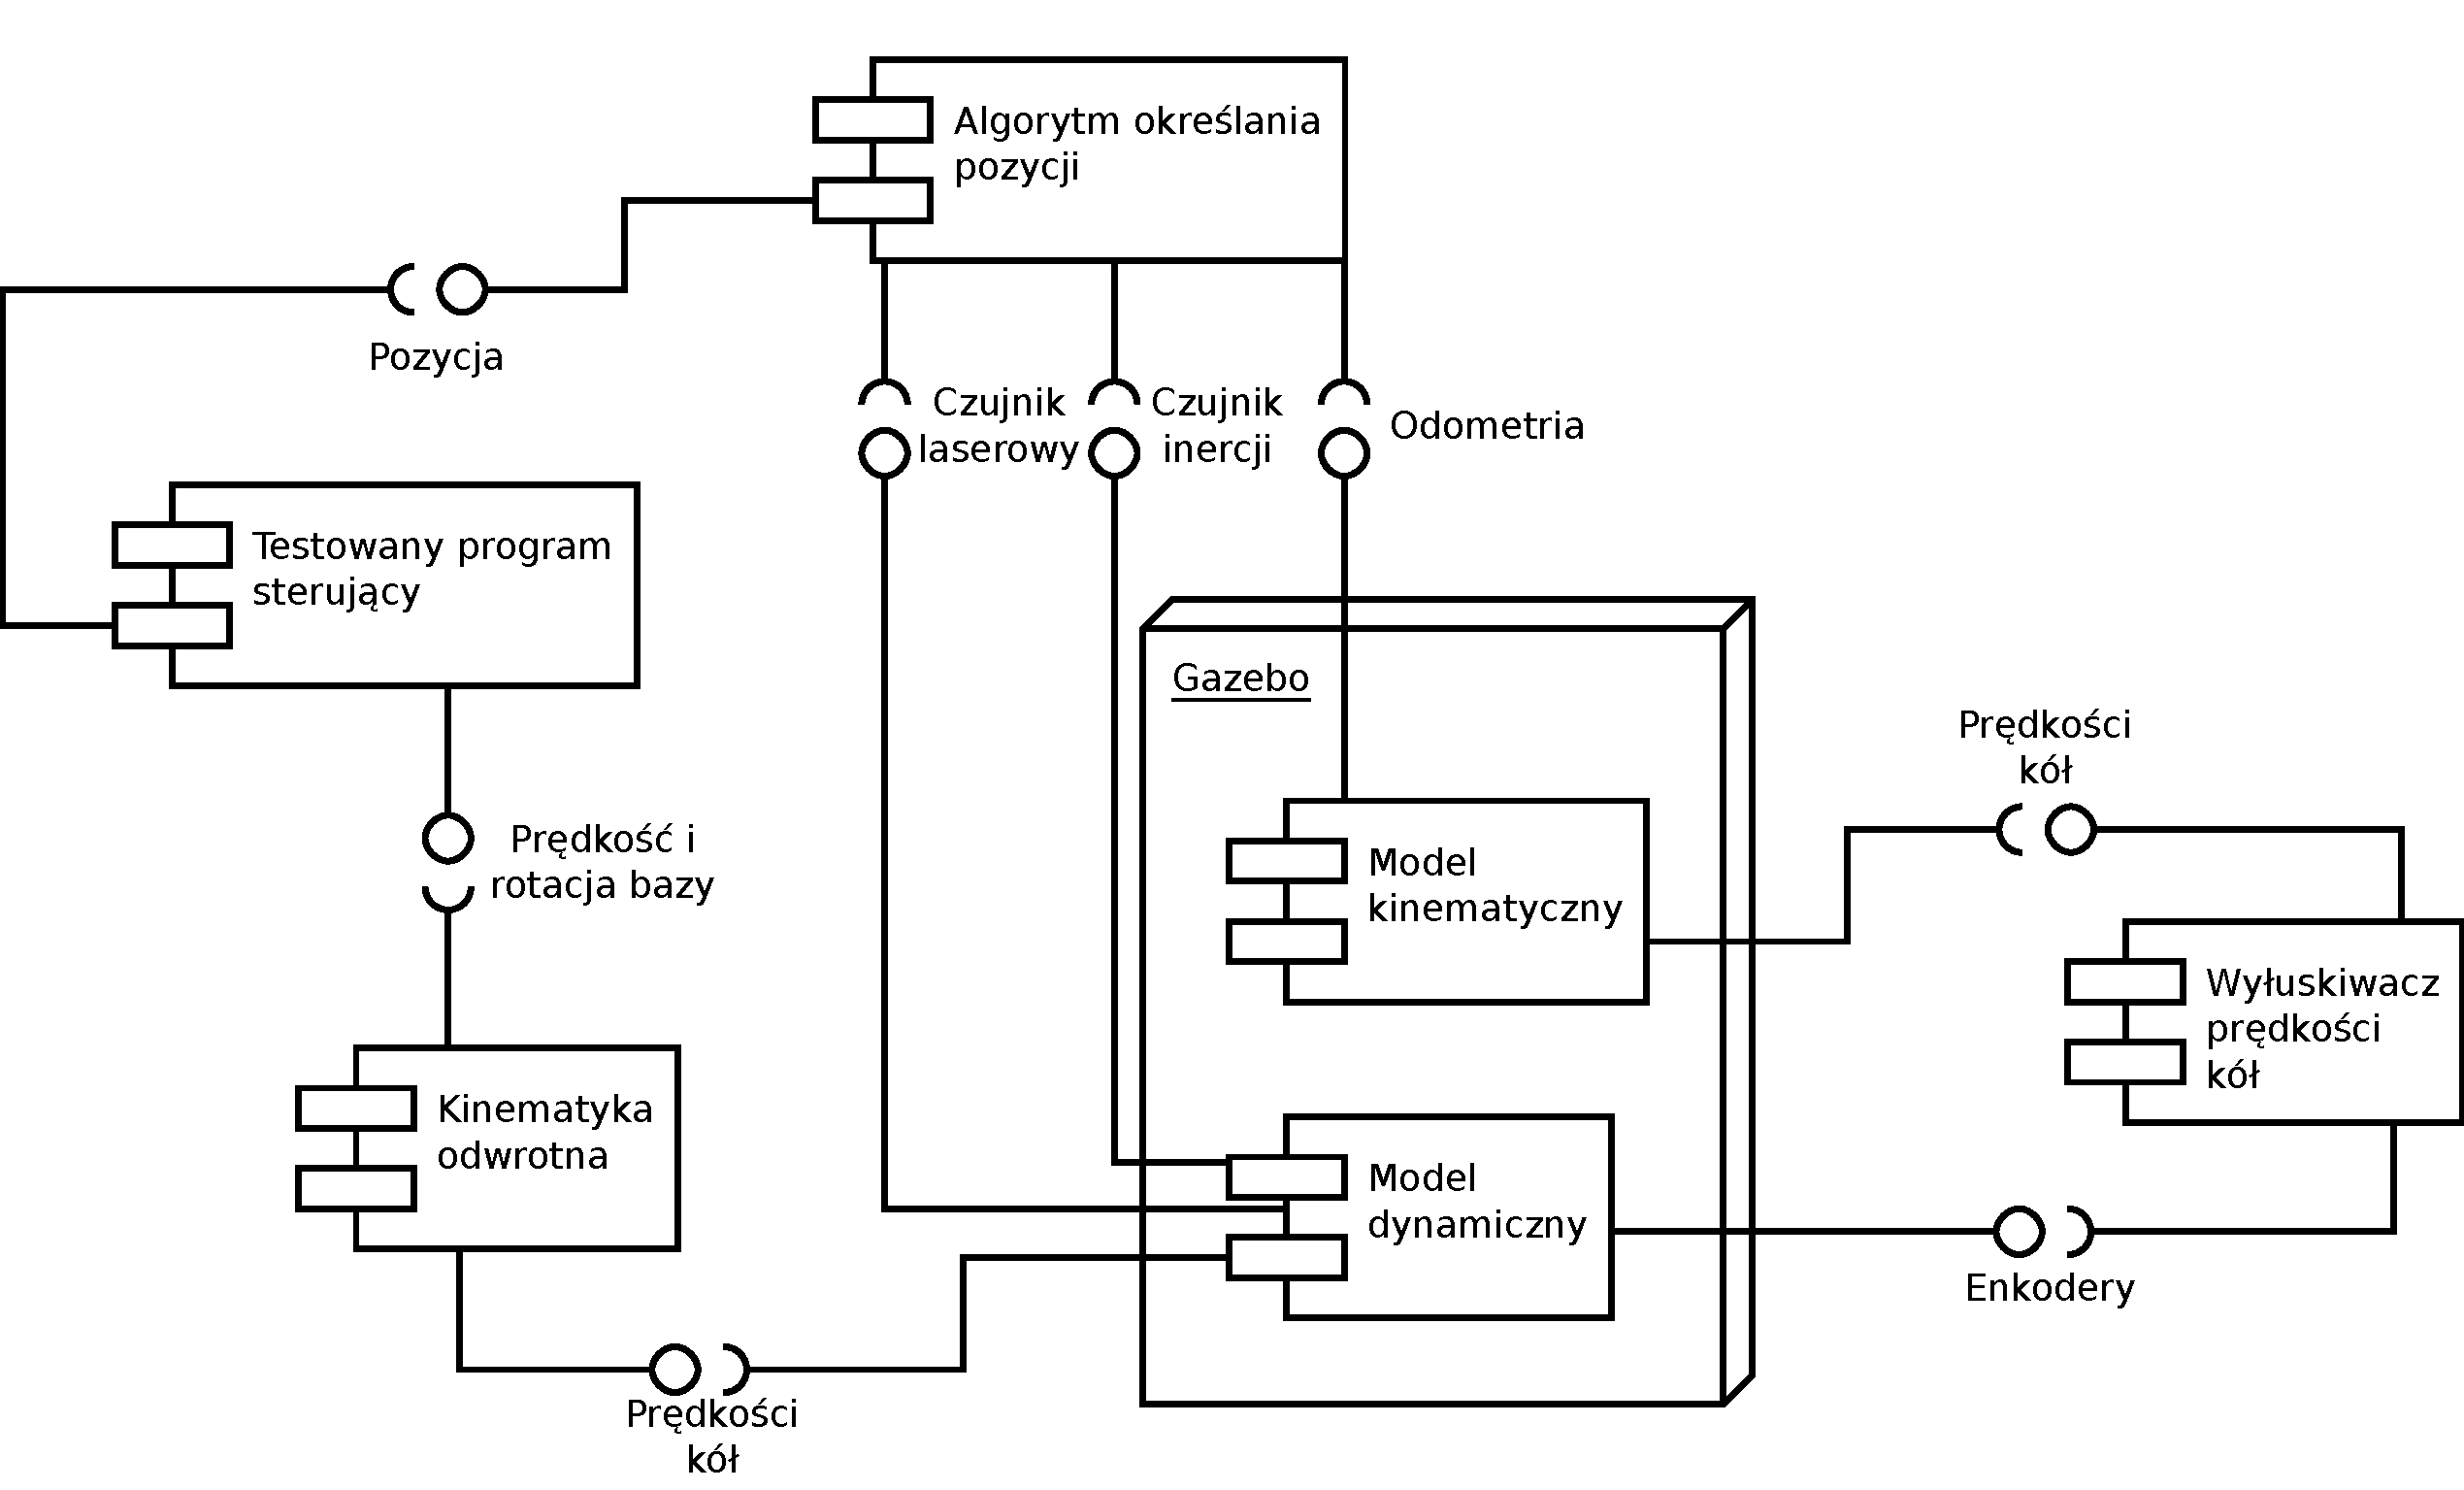
\includegraphics[width=\textwidth]{uml/final.pdf}
	\caption{Komunikacja podstawowych pakietów systemu w trakcie testowania programu sterującego.}
\end{figure}

Ważną rolę odgrywa tutaj algorytm określania pozycji, bazujący na odometrii, jednostce inercyjnej i danych ze skanera laserowego.
Odometria jest generowana za pomocą modelu kinematycznego, sterowanego danymi z enkoderów modelu dynamicznego.
Sam model dynamiczny sterowany jest pośrednio przez program, który generuje zadane prędkości i obrót robota.
W uproszczeniu: program sterujący wysyła sterowanie do modelu, bazując na jego pozycji, określonej z danych generowanych przez modele czujników.

W każdym miejscu przepływu danych można zebrać i zwizualizować przesyłane wartości.
Program sterujący może także korzystać ze skanerów laserowych w celu wykrycia przeszkody, nie tylko w celu określenia pozycji.
Bardziej zaawansowany program sterujący mógłby generować zadane prędkości kół bezpośrednio, nie bazować na modelu kinematyki odwrotnej.

\section{Zapis agentowy}
	Aby zachować kompatybilność programu sterującego platformy mobilnej z jej modelem, należy stworzyć efektory i receptory wirtualne, do których 
	program sterujący będzie wysyłał i z których będzie odbierał dane. 
	Te wirtualne byty będą dalej przekazywać informacje zarówno do modeli, jak i do robota w taki sposób, że
	główny program sterujący nie będzie miał żadnej informacji o tym, do czego jest podłączony. 
	
	\begin{figure}[H]
		\centering
		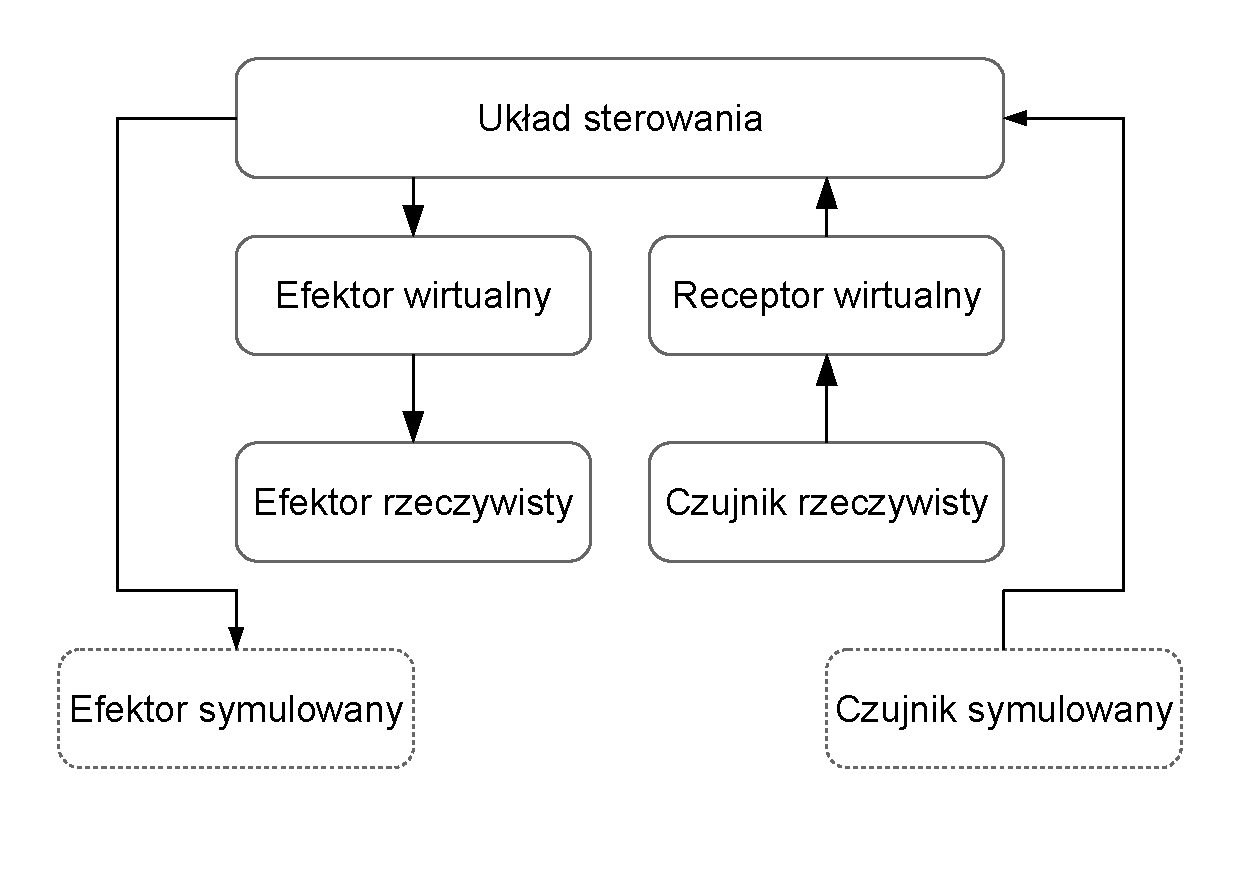
\includegraphics[width=0.8\textwidth]{graphics/agent.pdf}
		\caption{Struktura agenta upostaciowionego.}
		\label{fig:agent}
	\end{figure} 

	Można to przedstawić za pomocą zapisu agentowego, rysunek \ref{fig:agent}.
	Agent upostaciowiony składa się z kilku modułów, komunikujących się ze sobą za pomocą różnych interfejsów.

	Nadrzędnym modułem jest układ sterowania, który na podstawie odczytów z czujników generuje sterowanie dla efektorów.
	Ważne jest, aby komunikacja z rzeczywistymi urządzeniami była identyczna, jak z ich modelami, dzięki czemu taki system będzie przenośny i niezależny od implementacji modelu.

	Efektor rzeczywisty, na przykład serwomotor, jest sterowany za pomocą efektora wirtualnego, który zamienia wyjście układu sterowania na sygnały sterujące dla silnika napędowego.
	Przykładowo, zmienia odebraną liczbę, oznaczającą zadaną prędkość, na odpowiednie napięcie na wyjściu układu sterującego.

	Zamodelowany efektor symulowany również przyjmuje te same sygnały do układu sterowania, co efektor rzeczywisty, 
	lecz nie zamienia ich na sygnały sterujące, a wywołuje odpowiednie funkcje maszyny symulacyjnej, nadające siły i prędkości obiektom w przestrzeni wirtualnej.

	Receptor wirtualny pobiera surowe dane z czujnika, przekształca na odpowiedni format, usuwa błędy i szum tak, aby program sterujący mógł wykorzystać te dane w prosty sposób. 
	Doskonałym przykładem jest tutaj urządzenie Kinect (widoczne na robocie Velma na rysunku \ref{fig:velma}), w którym to zachodzi odczytanie obrazu z kilku kamer.
	Następnie obraz przesyłany jest do komputera, w którym sterowniki interpretują dane, usuwając błędy, tworzą mapę głębokości, wykrywają szkielety i sylwetki osób.
	Te dane mogą być wykorzystane łatwo w grach i programach sterujących.

	Modelowanie receptora, tak jak w przypadku efektora, polega na wygenerowaniu odpowiednich danych, używając odpowiednich funkcji w przestrzeni wirtualnej.
	Mogą one polegać na emitowaniu półprostych, symulujących laser, lub wręcz renderowaniu obiektów, aby uzyskać obraz z wirtualnej kamery.
	Receptor symulowany ma pełną wiedzę o symulowanym świecie, dokładne pozycje i prędkości wszystkich obiektów, dane o kolizjach itp. 
	Pozwala to na łatwe symulowanie receptorów nie mogących mieć odwzorowania w rzeczywistości, co przydatne jest w pierwszych stadiach testowania i wyznaczaniu statystyk.
	Takim przykładem jest model czujnika dokładnej pozycji, rotacji i prędkości w kartezjańskim układzie współrzędnych. 
	Czujniki typu GPS, lub żyroskopy nie generują tak dokładnych pomiarów.


\section{Model kinematyczny}
	\label{sec:pseudovelma}
	Kinematyka opisuje ruch obiektów bez rozważania sił powodujących ten ruch.
	Nie uwzględnia się przy opisie ruchu takich czynników, jak masa, moment bezwładności, czy siły.
	
	Model kinematyki określa równania prostego zadania kinematyki. 
	Rozwiązanie tego zadania polega na obliczeniu prędkości liniowej i kątowej bazy mobilnej na podstawie aktualnych prędkości kół.
	Symulator pozwala również na całkowanie tych prędkości, aby uzyskać aktualną pozycję platformy, z dokładnością do pozycji startowej.
	
	Równania modelu kinematyki najwygodniej przedstawić w postaci macierzowej, podobnej do tego, jak opisano w \cite{wheels}. 
	Dokładna podstać wzoru zależy od kolejności numerowania kół i interpretacji wymiarów.
	Dla opisanego tutaj przypadku, (stałe zdefiniowane są w tabeli \ref{tab:dims}, numeracja kół jest pokazane na rysunku \ref{fig:base_dims}):
	
	\begin{equation}
	\begin{bmatrix}
	v_x \\
	v_y \\
	\omega_z \\
	\end{bmatrix}
	=
	\frac{r}{4}
	\begin{bmatrix}
	-1 & 1 & -1 & 1 \\
	1 & 1 & 1 & 1 \\
	\frac{2}{a+b} & \frac{-2}{a+b} & \frac{-2}{a+b} & \frac{2}{a+b} \\
	\end{bmatrix}
	\begin{bmatrix}
	\omega_1 \\
	\omega_2 \\
	\omega_3 \\
	\omega_4 \\
	\end{bmatrix}
	\end{equation}
	
	Uzyskane wartości należy zastosować w funkcjach symulatora, aby nadać obiektom wirtualnym odpowiednie prędkości.
	
	Sterowanie pozycją modelu kinematycznego odbywa się wyłącznie poprzez powyższy wzór, zatem w jego symulacji nie uczestniczy maszyna symulacyjna fizyki.
	Ten model nie reaguje na kolizje z innymi obiektami, nie reaguje na różnicę terenu i nie używa informacji o współczynnikach tarcia materiałów.

	\subsection{Zachowanie}
		Platforma ignoruje inne obiekty znajdujące się na scenie,
		Po nadaniu stałych prędkości kół, następuje ruch zgodnie z rysunkiem \ref{fig:mecanum_dirs}.

		Program sterujący co każdy krok symulacji (okres zależy od zasobów procesorowych komputera) zwraca aktualne położenie i orientację, oraz prędkość liniową i kątową. 

\section{Model dynamiczny}
	\label{sec:omnivelma}
	Maszyna do symulacji dynamiki używa informacji o kształtach, masach i złączach pomiędzy ogniwami robota.
	Należy zatem stworzyć obiekt, złożony z modeli ogniw i samych ogniw i umieścić w symulatorze.
	Potem należy nadać obiektom odpowiednie siły, aby otrzymać wyniki przybliżone do tego, jak zachowywałaby się rzeczywista baza mobilna.

	Baza mobilna jest bryłą, na którą składają się następujące części składowe:
	\begin{itemize}
	\item Główna część korpusu.
	\item Ruchoma, mniejsza część korpusu, z przodu robota.
	\item 4 koła, 2 podłączone do głównej części korpusu, a 2 do przedniej.
	\item Po 12 rolek na każdym kole.
	\item Przegub obrotowy, łączący dwie części korpusu.
	\item 4 przeguby obrotowe z silnikami, łączące części bazy z kołami.
	\item 12 przegubów obrotowych na każdym kole, łączących koła z rolkami.
	\end{itemize}

	Jest to dość złożony obiekt do symulacji, dlatego należy dążyć do uproszczenia modelu, w celu zmniejszenia ilości obliczeń symulatora.
	Istnieje wiele podejść do stworzenia odpowiedniego modelu, na przykład jak najdokładniejsze odwzorowanie budowy platformy 
	za pomocą wzorów różniczkowych \cite{braking} \cite{modelling_ways}.
	
	\subsection{Zachowanie}
		Model reaguje na siły przyłożone do jego ogniw, porusza się, reagując na otoczenie.
		Bierze udział w kolizjach, nadaje prędkości innym obiektom.
		Współczynniki tarcia podłoża i kół mają znaczenie w symulacji.
		Powstają niedokładności wyznaczania pozycji, spowodowane dużą ilością zmiennych, uczestniczących w symulacji i precyzją symulatora.
	
\section{Model skanera laserowego}
	\label{sec:monokl}
	Symulator generuje odpowiednie dane, emitując promienie w przestrzeni wirtualnej.
	Następnie maszyna symulacyjna fizyki oblicza kolizje promieni z obiektami na scenie.
	Jest to operacja bardzo kosztowna obliczeniowo.
	
	Do położeń punków dodawany szum o rozkładzie normalnym, aby symulować błędy pomiarowe, powstałe przy odczycie odbicia lasera.
	
	Odczyt z rzeczywistego skanera pokazuje, że sztucznie wygenerowane dane są podobne do danych zebranych przez czujnik.
	Dodatkowo, wbudowany w czujnik sterownik usuwa błędy grube z pomiarów, zatem rzeczywiste dane nie posiadają ich, więc i nie jest konieczne dodawanie ich do modelu.
	
\section{Model jednostki inercyjnej}
	Rzeczywisty czujnik obarczony jest bardzo dużymi błędami pomiarowymi.
	Jednakże, jego model także zwraca bardzo zaszumiony obraz.
	
\section{Model kinematyki odwrotnej}
	\label{sec:transmutator}
	Jest to model kinematyki odwrotnej, alternatywa do modelu kinematycznego, opisanego w sekcji \ref{sec:pseudovelma}, jednak działającego bez symulatora i bez możliwości 
	całkowania prędkości (i generowania danych o aktualnej pozycji).
	Całkowanie prędkości kół i tak nie ma większego sensu, ponieważ pozwoliłaby jedynie obliczyć aktualną ich pozycję.
	Z wyjątkiem porównania tych danych z danymi z enkoderów, nie ma to zastosowania.
	
	Ten pakiet przyjmuje zadaną prędkość, kierunek i obrót platformy, a zwraca prędkości kół, które powinny być nadane platformie, aby wywołać taki ruch.
	Wzory mogą być przedstawione w postaci macierzowej.
	
	\begin{equation}
	\begin{bmatrix}
	\omega_1 \\
	\omega_2 \\
	\omega_3 \\
	\omega_4 \\
	\end{bmatrix}
	=
	\frac{1}{r}
	\begin{bmatrix}
	1 & -1 & \frac{a+b}{2} \\
	1 & 1 & -\frac{a+b}{2} \\
	1 & -1 & -\frac{a+b}{2} \\
	1 & 1 & \frac{a+b}{2} \\
	\end{bmatrix}
	\begin{bmatrix}
	v_y \\
	v_x \\
	\omega_z \\
	\end{bmatrix}
	\end{equation}
	
	Stałe, użyte we wzorze zdefiniowane są w tabeli \ref{tab:dims}, a numerowanie kół na rysunku \ref{fig:base_dims}.
	Ten wzór, podobnie jak poprzedni, pojawia się w wielu pracach, na przykład \cite{wheels}, dokładny wygląd macierzy zależy od numerowania kół i interpretacji kierunków osi.
	
	Dodatkowo, program pozwala na obrót wektora prędkości o kąt prosty, lub półpełny. 
	Jest to spowodowane tym, że różne pakiety i różne modele przyjmują różną pozycję wyjściową robota.
	Czasami przód modelu skierowany jest w dodatnią stronę osi X, a czasami Y. W związku z tym, ta funkcjonalność jest w stanie przekonwertować dane wejściowe dla innego robota tak,
	aby mogły być użyte do sterowania opisywanym tutaj robotem.
	

\section{Manualne sterowanie}
\label{sec:lalkarz}
	To zaawansowany program do manualnego generowania zadanych prędkości kół, lub prędkości liniowej i kątowej platformy.
	Ponieważ jest niezależny od reszty systemu, może być użyty do sterowania rzeczywistym robotem.
	Pozwala także na wyświetlanie aktualnych prędkości kół, generowanych przez enkodery.
	
	Sterowanie można nadać poprzez klawiaturę, kontroler do gier, lub myszkę.
	Program otwiera graficzne okno, w którym wyświetla aktualne dane i wskaźniki prędkości.
	
\section{Generator sterowania}
	\label{sec:gramofon}
	Podstawą przeprowadzania testów modelu jest powtarzalność eksperymentów, oraz dokładność nadanego sterowania.
	Potrzeba zatem jest sposobu na automatyczne wygenerowanie strumienia wiadomości z określonymi danymi.
	
	Ten pakiet generuje powtarzalne sterowanie, bazując na wczytanym pliku tekstowym.
	Zwraca zadane prędkości liniowe i prędkość kątową bazy.
	
	Podłączono go do rzeczywistego robota, aby poruszał platformą po kwadracie i obracał wokół osi.
	Eksperyment przebiegł pomyślnie.
		
\section{Wyłuskanie struktury wiadomości}
	\label{sec:dziadzio}
	Każda wiadomość przekazywana pomiędzy węzłami jest zwykle zagnieżdżoną strukturą.
	
	Czasami może zdarzyć się, że jakiś węzeł potrzebuje jedynie wewnętrznej podstruktury wiadomości.
	Nie powinno mu się zatem przekazywać całej struktury wiadomości, gdyż to powodowałoby niepotrzebne opóźnienia, oraz nie pozwoliłoby zachować niezależności 
	pakietu od innych.
	
	Takie zjawisko występuje przy przekazywaniu informacji o pozycji i prędkości kół, generowanej przez model czujnika enkoderów, do programu
	manualnego sterowania, lub przekazywanie danych z enkoderów do modelu kinematycznego.
	
	ROS nie pozwala na automatyczne odbieranie tylko części pakietu, dlatego powstał ten program.

\section{Podłoże o zmiennym współczynniku tarcia}
	\label{sec:flooria}
	Symulacja nie składa się jedynie z robota i czujnika, ale także z podłoża, na którym musi się poruszać.
	Ponieważ podłoże również wpływa na symulację, powinien istnieć sposób na ustawienie jego współczynnika tarcia.
	
	Ten pakiet jest modelem ładowanym do symulatora Gazebo, przyjmuje on asynchroniczne wywołania, nadające podłożu odpowiednie tarcie.
	W ten sposób można testować zachowanie się modelu w różnych przypadkach testowych.
	
\section{Algorytm usuwania szumu z danych jednostki inercyjnej}
	\label{sec:odszumiacz}
	Jak wcześniej wspomniano, jednostka inercyjna i jej model zwracają bardzo duże błędy pomiarowe.
	
	Ten program uśrednia dane w prosty sposób, licząc średnią z określonej ilości poprzednich pomiarów.
	Taki algorytm nie sprawdza się jednak, gdy dane są generowane naprzemiennie.
	Na przykład, jeśli w jednej klatce symulacji maszyna do symulacji fizyki obliczy prawidłową wartość, a w drugiej zwróci zerową,
	to ten algorytm uśredni te wyniki i zwróci wartość pośrodku. Działa to bardzo dobrze przy uśrednianiu 
	szumu przy zerowym przyspieszeniu, w trakcie ruchu robota z prędkością jednostajną.
	
	W przyszłości zastosować trzeba będzie bardziej zaawansowany algorytm uśredniania odczytów.
	Może on być również testowany na tym modelu.
	
	Stworzenie tego modułu pozwoliło zbadać, czy model jednostki inercyjnej reaguje na ruch platformy w odpowiednim kierunku, gdyż
	pomiary są obarczone tak dużymi błędami, że wizualizacja odczytów na wykresie nie daje gwarancji upewnienia się o działaniu modelu.
	
\section{Obserwator symulacji}
	\label{sec:ocznica}
	Model uruchamiany w symulatorze.
	Oblicza i zwraca statystyki międzymodelowe w przestrzeni symulacji, takie jak odległość i kąt.
	Pozwala zbadać, jak model dynamiczny zachowuje się w stosunku do modelu kinematycznego, to znaczy, 
	czy pozycja, obliczone przez maszynę symulacyjną fizyki jest zbliżona do pozycji obliczonej równaniami kinematycznymi po całkowaniu.
	
\section{Scena z symulacją}
	Symulator Gazebo przy uruchomieniu ładuje plik zawierający referencje robotów i ich początkowe pozycje, używane w symulacji.
	Ten pakiet nie jest programem wykonywalnym, lecz prezentuje informacje dla symulatora o scenie symulacji.
	
	
	W tym pliku zawierają się także ustawienia symulacji, jak przyspieszenie grawitacyjne, typ maszyny symulacyjnej fizyki ze współczynnikami, czy ustawienia wirtualnej atmosfery.
	
\section{Rozdzielacz pakietów}
	Jeśli dwóm węzłom nadać te same nazwy interfejsów strumienia wiadomości, to ROS będzie przekazywał pomiędzy nimi informacje.
	To jednak nie zawsze jest możliwe, aby mieć całkowitą kontrolę nad nazwami interfejsów wszystkich węzłów.
	Dlatego też, potrzebny jest program do przekazywania i ewentualnego rozdzielania wiadomości dla różnych odbiorników.
	
	Ten program wykonywalny pobiera i generuje wiadomości zawierające zadane prędkości kół.
	Pozwala to na sterowanie kilkoma robotami o identycznym interfejsie ze wspólnego źródła.
	W szczególności przydaje się to przy rozdzielaniu wartości prędkości kół dla modelu platformy dynamicznej i kinematycznej.
	
\section{Prosty program sterujący}
	Jest to uproszczona wersja programu, który docelowo ma być tworzony na podstawie budowanego systemu modeli.
	Pozwala on sprawdzić, jak dla prostych zasad model będzie się zachowywał.
	
	Program periodycznie wysyła dane o zadanej prędkości.
	W zależności od danych z czujników laserowych, program zmienia swój stan i obraca kierunek obrotu o 90\textdegree.
	Ten sterownik dla uproszczenia nie generuje poleceń obrotu kątowego, sterowany obiekt powinien zachować swoją orientację.
	
	Prosty algorytm programu gwarantuje omijanie przeszkód, aby platforma nie zderzyła się z jakimś obiektem, jednak nie bierze pod uwagę celu jazdy.
	To znaczy, że platforma będzie poruszać się od przeszkody do przeszkody w losowy sposób.
	
\section{Struktury pakietów wiadomości}
	Ten pakiet nie jest plikiem wykonywalnym, a definicjami struktur danych, używanych przez wiadomości ROSa w projekcie, jeśli 
	standard nie obejmuje potrzebnego typu wiadomości.
	
	Dodatkowo zdefiniowane typy wiadomości to:
	\begin{itemize}
		\item Dane prędkości i rotacji kół, zwracane przez model enkoderów.
		\item Dane o względnej pozycji i rotacji obiektów na scenie.
		\item Zadane prędkości kół.
		\item Asynchroniczne wywołanie do ustawienia inercji ogniw modelu.
		\item Asynchroniczne wywołanie do ustawienia współczynników tarcia.
	\end{itemize}

\section{Zewnętrzne pakiety ROSa}
	Istnieje kilka tysięcy różnych pakietów i programów, tworzonych przez społeczność ROSa.
	
	\subsection{Rysownik wykresów}
		Pakiet \texttt{rqt-multiplot} jest wtyczką do większego programu \texttt{rqt}.
		Pozwala na generowanie dwuwymiarowych wykresów, bazując na dwóch dowolnych wartościach z odbieranych pakietów, lub czasie.
		Można porównać różne wykresy na jednym układzie.
		
		W szczególności, przy ustawieniach pozycji Y względem X, pobranych z pakietu pozycji, nadawanego przez obie platformy, pozwala narysować trajektorię ruchu platform.
		
	\subsection{Wizualizer pomiarów}
		Oryginalnie napisany dla robota o tej samej nazwie, \texttt{rviz} prezentuje trójwymiarową przestrzeń, na której można wyświetlać 
		dane odebrane z innych węzłów.
		
		Pozwala to na przykład umieścić znacznik reprezentujący pozycję platformy i chmury punktów, odebranych z czujników laserowych.
		Jest lżejszy na zasobach w działaniu niż Gazebo i pokazuje tylko informacje z odebranych danych, a nie całe środowisko symulacji.
		Nie posiada własnego symulatora fizyki, nie generuje żadnych danych samodzielnie.
		
	\subsection{Zbieranie danych}
		Każdy strumień wiadomości może zostać zapisany do pliku, a następnie odtworzony w ten sam sposób, w jaki został odebrany.
		Wbudowane w ROSa narzędzie \texttt{rosbag} pozwala ,,nagrać'' i odtworzyć dane.
		Zapisuje to w formie pliku binarnego, wraz z dokładnymi parametrami działania nadajnika wiadomości, takimi jak nazwy ścieżek, ilość odebranych wiadomości, czas.
		
		Korzystając z pomocniczego narzędzia do zarządzania węzłami, \texttt{rostopic},
		możliwe jest również wydrukowanie danych do pliku tekstowego w formacie CSV (\emph{Comma Separated Values}),
		aby mogły być następnie wykorzystane w dowolny sposób przez inne programy jak Gnuplot, Calc (Exel), czy Matlab.
		
	
	
	
	
	

